
\addcontentsline{toc}{section}{Введение}

\section*{Введение}\label{intro}

Индуцирование плазмонного резонанса в системе с напылением проводящего слоя на диэлектрики различной конфигурации (призма или цилиндр ) открывают возможность создать очень чувствительный к внешним параметрам сенсор.

Физическое явление которое легло в основание данной схемы было предложено Кречманом и Отто. Для производства сенсоров наиболее применимой и удобной является схема Кречмана которая является фундаментом для построения схемы расмотренной в данной работе.
Световой пучок падает на сэндвич из диэлектрика с $ \varepsilon_p >1 $ и слоя с металлическим напылением испытывая полное внутренне отражаение. В идеалированной ситуации коэффицент отражения равен единице, однако при некотором угле падение возникает резкое падение коэффицента отражения вызванное скачком интенсивности поля у металла. В литературе это называют нарушенным полным внутренним отражением (НПВО).

Данная конфигурация очень полезна так-как позволяет посчитать $ \varepsilon $ среды граничащей с металлом по расположению скачка коэффицента отражения из-за чувствительности данной схемы к свойствам материала.

В данной же работе будет исследована цилиндрическая конфигурация с наклонной брегговской решёткой.

\begin{figure}[h!]
	\centering
	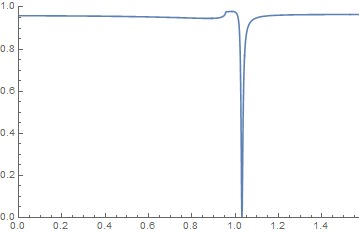
\includegraphics[width=0.5\linewidth]{kretchmann}
	\caption[Эффект Кречмана]{}
	\label{fig:kretchmann}
\end{figure}







\section*{Благодарности}\label{ty}

В первую очередь, хочется поблагодарить моего научного руководителя А.В. Дорофеенко без которого было бы невозможным написание данной работы и чья неоценимая помощь и руководство помогли её завершить. Автор также признателен А.П. Виноградову за лекции по электродинамике композоитов прочтённые им в ИТПЭ, которые помогли сформировать представления автора об этой новой области науки и чьи наставления значительно повлияли на мирощущение автора. Особенную благодарность заслуживает А.А. Пухов, сыгравший ключевую роль в образовании и становлении автора как учёного, за его лекции по квантовой механике, статистической физике, колебаниям и волнам живая и интересная подача которых возбудила неутомимый интерес автора к теоретической физике. Его вера в автора не давала сдаваться перед лицом трудностей, а благочестивые нравоучения направляли на пути познания. Кроме того, автор благодарен А.М. Мерзликину
за очень содержательные и познавательные семинары предмет которых затруднительно вспомнить. 


\pagebreak[4]